\chapter{Conceptual Extensions}\label{title:concept}
In this chapter, we first give an overview over the current state of invariant generation and usage in \CPAchecker{}. Then, we introduce some new concepts to improve the handling of 
invariants and also explain some additional approaches to invariant generation.

\section{Architecture before this Thesis}\label{title:arch_old}
Before this master's thesis, auxiliary invariants were mainly used for analyses doing \Kinduction{} in \CPAchecker{}. The only other use-case were path invariants, which also rely on 
\autoref{alg:continously-refined} for generating invariants. In \autoref{fig:arch_before},  the most important parts for generating and retrieving invariants in \CPAchecker{} are displayed.

\begin{figure}
 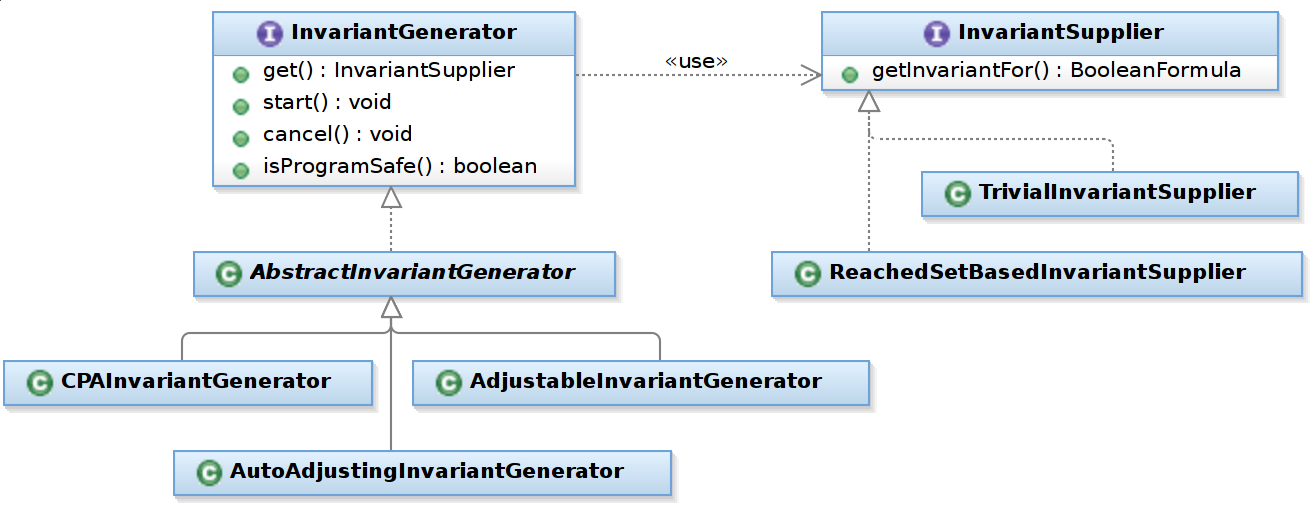
\includegraphics[width=\textwidth]{../graphics/invgen_arch.png}
 \caption{Invariant generation in \CPAchecker{} (old)}
 \label{fig:arch_before}
\end{figure}

There are several implementations of the \texttt{InvariantGenerator} interface. First there is the \texttt{CPAInvariantGenerator}, a class that uses a given \ac{CPA} and \autoref{alg:cpa}
without the possibility of adding \ac{CEGAR} or continously-refined invariants.

Then there is the \texttt{AdjustableInvariantGenerator}, which can be wrapped around any \texttt{CPAInvariantGenerator}, and more importantly, which can be used to adjust some conditions of
the invariant generation, for example, resetting the reached set to only contain the initial state, and increasing the precision before restarting the $\CPAAlgorithm{}$. The
\texttt{AutoAdjustingInvariantGenerator} is a wrapper around an \texttt{AdjustableInvariantGenerator}. With this implementation, the given function to adjust the invariant generation is
called automatically upon a finished invariant generation run, and then invariant generation is started again. This is done in a loop until either the invariant generation is cancelled or
the invariant generator proved the safety of the program.

Besides the \texttt{CPAInvariantGenerator}, all invariant generator implementations are package private and therefore hidden from users.
Using them is only possible via the \texttt{CPAInvariantGenerator} by setting the corresponding configuration options.
Moreover, invariant generation can be either executed sequentially, or it can be run in parallel on a separate thread\,\sidenote{For both
options calling the \texttt{start} method starts the invariant generation.}.
The method \texttt{isProgramSafe} indicates if the invariant generator was able to prove the safety of a program. In the case that safety was proved by
the invariant generator, we can stop the overall analysis and return that the program is safe.
This is not easily possible, as according to \autoref{alg:cpa} the returned value of an analysis is its reached set, which either
contains an error state (the program is unsafe) or does not contain an error state (the program is safe). From inside the \ac{CPA} we can however not change the returned reached set. This 
is only possible in the algorithm. Therefore, the only possible option is to remove all currently contained error states from the reached set of the \ac{CPA} and additionally removing
all states from the waitlist.
A weakness of this approach is, that the returned reached set does not contain the information that the specification violations in the the program are not reachable. And even worse the
violations would be found again if we do not manually remove all pending states from the waitlist\,\sidenote{Instead of the reached set of the primary analysis it would be better to
return the reached set of the invariant 
generator, which is however not possible with the current available algorithms.}. Thus, we have an invalid reached set as result of the analysis in the case we want to use the shortcut as soon as
the invariant generator proved safety.

Another drawback of the current invariant generation is the encoding of the invariants. According to the \texttt{InvariantSupplier} interface, an invariant is always a 
\texttt{BooleanFormula}\,\sidenote{A BooleanFormula is always an \ac{SMT} formula, from our \ac{SMT} backend JavaSMT, cf. \url{github.com/sosy-lab/java-smt}}. This restricts the use of the 
invariant generator to analyses based on \ac{SMT} formulas and more importantly, the formulas need to be encoded in the same way in both analyses, otherwise they cannot be combined. As an example, it 
is sufficient to consider an analysis that works with bit-precise \ac{SMT} formulas, and an invariant generator that only approximates values using unbounded integers. Even if the naming of the variables 
in the formulas generated by the invariant generator is equal to the one of the primary analysis, due to the different types, the invariants are unusable. While this is a quite obvious 
requirement, there are also some hidden pitfalls, especially when it comes to pointer aliasing. In the following two sections, we will introduce our conceptual additions to overcome all 
mentioned problems, and also show our implementation of these additions.



\section{Reached Set-based Data Exchange between Analyses}\label{title:concept_reached}
As mentioned in the last section, due to the return type of the interface \texttt{InvariantSupplier}, using auxiliary invariants in \CPAchecker{} is strongly tied to \ac{SMT}-based analyses.
There, each analysis that is supposed to use invariants generated with an \texttt{InvariantGenerator} implementation needs to know internal information about the encoding of the formulas
to be able to use the invariants correctly.

By removing the \texttt{InvariantSupplier} completely, and instead returning the generated reached set when \texttt{get} is called on an instance of \texttt{InvariantGenerator}, we solve
the problem of invariants being only usable within \ac{SMT}-based analyses\,\sidenote{For better encapsulation the return type of \texttt{get} will not be a reached set but a wrapper around one 
or more reached sets. More information on this can be found in \autoref{title:architecture_final}.}. By retrieving all states for a certain location from the reached set, each consumer can then 
create the invariant in any encoding --- \ac{SMT}-based or not --- individually.

While in principle this solves all encoding related problems, and makes invariants usable for all analyses in \CPAchecker{}, the handling of the invariant encoding was just moved 
to another location. Before our changes, implementations of the \texttt{InvariantSupplier} interface had to take care of the encoding such that it matches the encoding of the Predicate 
CPA\,\sidenote{The \PredicateCPA{} was the only analysis which used invariants in combination with \Kinduction{}.}. Now, because we do not have the invariant as a \texttt{BooleanFormula}, but instead 
we have the reached set, we need to do the transformation ourselves in an appropriate place. For that reason, we added the \texttt{FormulaInvariantSupplier}, a wrapper class for reached 
sets, which computes the invariant depending on given parameters such as the location or the information about pointer aliasing.

The next section shows a further generalization of asynchronous invariant generation in \CPAchecker{} that is also based on analyses exchanging reached sets.
Synchronous invariant generation --- before the consuming analysis is run --- is also possible. Therefore we extend the sequential combination of analyses
(cf. \autoref{title:restart}) such that the reached set of an analysis that was run prior to another analysis can be used in the later analysis.

\section{Parallel Analyses}
Besides the encoding and the limitation of invariants to having the type \texttt{BooleanFormula}, another problem with the implementation of the invariant generation in \CPAchecker{} is that
if an invariant generator proves safety we could potentially use its result as a shortcut, instead of the result of the primary analysis. However from inside the \ac{CPA} in a 
$\CPAAlgorithm{}$ it is not possible to return something else than the reached set used by this \ac{CPA}. Therefore we create an algorithm that has the following abilities:

\begin{enumerate}
 \item It wraps several analyses that will be executed in parallel.
 \item It allows distributing \emph{finished} reached sets\,\sidenote{Usually each analysis results in one reached set. By using a variation of \autoref{alg:continously-refined} an analysis could return more reached sets, with increasing precision.} to other, running, analyses.
 \item It takes the first \emph{valid} reached set\,\sidenote{The validity of a reached set depends on the soundness of the analysis, \eg, 
 for soundness the waitlist has to be empty if no target state is in the reached set, because if the waitlist is not empty we have not fully explored the state space, and can therefore not be sure that further exploration does not result in finding a reachable specification violation.} of its component analyses, returns it, and aborts all other analyses, because their results are no longer important.
\end{enumerate}

\SetKwFor{Parallel}{For}{do in parallel}{EndParallel}
\begin{algorithm}
\LinesNumbered
\SetKw{Var}{Variables}
\SetKw{Var}{Variables}
 \SetKwInput{Kw}{Variables}
 \KwIn{a list $L$ of quadruples with the following components:
       \begin{enumerate}
       \item a configurable program analysis with dynamic precision adjustment $\mathbb{D} = (D, \precision, \transabs, \mergeop, \stopop, \precop)$,
       \item a set $R_0 \subseteq (E \times \precision)$ of abstract states with precision,
       \item a subset $W_0 \subseteq R_0$ of frontier abstract states with precision, where $E$ denotes the set of elements of the semi-lattice of $D$,
       \item and a boolean flag that shows if the analysis should be continuously-refined
       \end{enumerate}}
 \KwOut{the set $\reached$ and the set $\waitlist$}
 \Kw{a set $\reached$ of elements of $E \times \precision$,\newline
     a set $\waitlist$ of elements of $E \times \precision$,\newline
     thread-local versions of both variables,\newline
     a thread-safe set $\mathsf{aggregated}$ of sets $\reached$ for communication between analyses}

 $\mathsf{aggregated} := \{\}$

 \Parallel{each $(CPA, R_0, W_0, refined) \in L$}{
   \eIf{$refined$}{

    \Loop{}{
      $\reached := \CPAAlgorithm(CPA, R_0, W_0)$\;
      $R_0 := \{(e, \mathtt{RefinePrec}(\pi)) | (e, \pi) \in R_0\}$\;
      $W_0 := \{(e, \mathtt{RefinePrec}(\pi)) | (e, \pi) \in W_0\}$\;
      \If{$\waitlist \iff \emptyset$}{
	$\mathsf{aggregated} := \mathsf{aggregated} \cup \{\reached_{thread}\}$\;
      }
      \If{$\neg \mathtt{containsTargetState}(\reached_{thread})$}{
	$\reached := \reached_{thread}$\;
	$\waitlist := \waitlist_{thread}$\;
	$\mathtt{cancel\_other\_threads}()$\;
	break\;
      }
    }
   }{
    $\reached_{thread} := \CPAAlgorithm(CPA, R_0, W_0)$\;
    \If{$\waitlist \iff \emptyset$}{
      $\mathsf{aggregated} := \mathsf{aggregated} \cup \{\reached_{thread}\}$\;
    }
    $\reached := \reached_{thread}$\;
    $\waitlist := \waitlist_{thread}$\;
    $\mathtt{cancel\_other\_threads}()$\;
   }
  }
   $\mathtt{join}()$\;
 \Return{$(\reached, \waitlist)$}
 \caption{$\ParallelAlgorithm{}$}
 \label{alg:parallel}
\end{algorithm}


Item 1 and 2 provide the basic feature of having an asynchronously running analysis, like it exists in \texttt{CPAInvariantGenerator}. Out of the finished reached sets, invariants can be 
computed. The feature of having continuously-refined invariants implemented within the class \texttt{AutoAdjustingInvariantGenerator} is also available in the new $\ParallelAlgorithm{}$ 
(cf. \autoref{alg:parallel}). For ease of presentation, we assume that all analyses are sound and precise and therefore no extra handling is required. In the implementation, soundness (no 
target states missed) and precision (target states are really target states) of an analysis are taken into consideration. If some conditions are not matching, \eg, the analysis is unsound 
but no specification violation was found, we ignore the result of this analysis and use the result of another of the concurrently running analyses if available.

Instead of invariants, the reached sets out of which the invariants can be extracted are given by the variable  $\mathsf{aggregated}$. The invariants can be retrieved orthogonally to 
$\mathtt{getCurrentlyKnownInvariants}$ from \autoref{alg:continously-refined}. While in the $\CPAAlgorithm{}$ no specific retrieval of reached sets is specified, we consider 
that calling this method will be up to the \acp{CPA} and can, for example, be done in the transfer relation. The method $\mathtt{containsTargetState}$ is the same as for \autoref{alg:continously-refined}. The 
methods $\mathtt{cancel\_other\_threads}$ and $\mathtt{join}$ are used for canceling concurrently running analyses, and for waiting on each concurrently running analysis to stop.

Overall, the refactoring of extracting the asynchronous invariant generation into the more generic $\ParallelAlgorithm{}$ has two major benefits. First, if safety can be proved with the 
invariant generator, we can use it without the need of incomplete reached sets (cf. \autoref{title:arch_old}). Second, the combination of several analyses (all of them can potentially be used 
as invariant generators) in parallel was not possible before, but is now. This can, \eg, be used like a sequential combination of analyses, with the difference that these 
analyses are run in parallel. 

\clearpage
\section{Architecture after this Thesis}\label{title:architecture_final}
With the new concepts introduced in the last sections, some changes to the software architecture of \CPAchecker{} become necessary. First, we need to implement the 
$\ParallelAlgorithm{}$\,\sidenote{See \autoref{fig:CPAchecker_architecture} for the alignment of this algorithm in \CPAchecker{}.} and a thread-safe means for exchanging reached sets,
called \AggregatedReachedSets{} in this thesis. Additionally, we have added the possibility 
of passing an \AggregatedReachedSets{} object, from one analysis to the next, in a sequential combination of analyses. Due to our changes the asynchronous invariant generation
can now be done as a parallel analysis. Therefore we can remove this functionality and the classes that are responsible for the (automatic) adjustment of 
the analysis from the former \texttt{InvariantGenerator} implementation. The only feature which is still available via the \texttt{CPAInvariantGenerator} is running an analysis sequentially. This feature is different to a sequential combination of 
analysis because the \texttt{CPAInvariantGenerator} can be run on the fly inside another analysis. This is, for example, important for path invariants later on.

\begin{figure}
  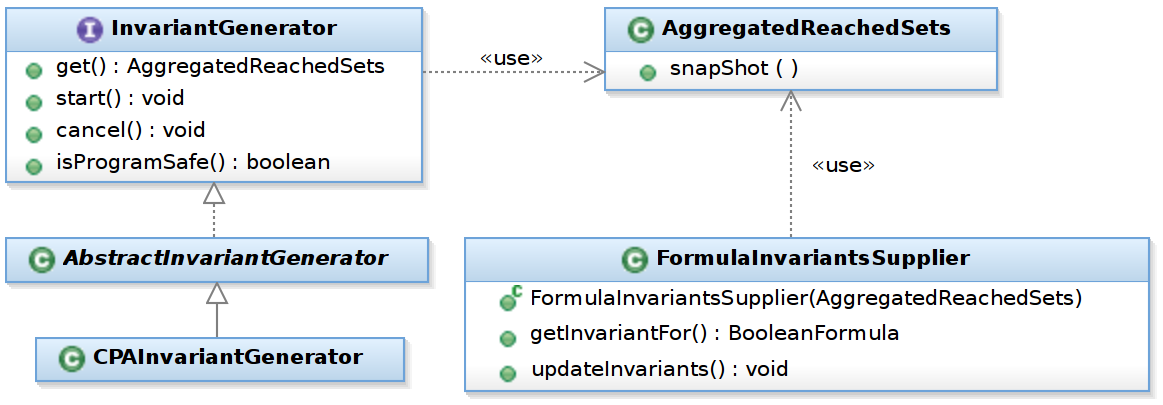
\includegraphics[width=\textwidth]{../graphics/invgen_arch_new.png}
 \caption{Invariant generation for \acs{SMT}-based analyses (new)}
 \label{fig:arch_after}
\end{figure}

\autoref{fig:arch_after} shows how invariants for \ac{SMT}-based analyses can be computed. The structural alignment of the $\ParallelAlgorithm{}$ can be found in 
\autoref{fig:CPAchecker_architecture}. In addition to the functionality shown in \autoref{alg:parallel}, the implementation is able to exclude certain reached sets from the 
\AggregatedReachedSets{}, such that they are only used as direct return values of the $\ParallelAlgorithm{}$ if applicable. The same applies to the sequential
combination of analyses, where one can configure that later analyses use reached sets of the earlier executed analyses. 

